\documentclass[12pt,a4paper]{article}
\usepackage{ctex}
\usepackage{amsmath,amscd,amsbsy,amssymb,latexsym,url,bm,amsthm}
\usepackage{epsfig,graphicx,subfigure}
\usepackage{enumitem,balance}
\usepackage{wrapfig}
\usepackage{mathrsfs,euscript}
\usepackage[usenames]{xcolor}
\usepackage{hyperref}
\usepackage[vlined,ruled,linesnumbered]{algorithm2e}
\usepackage{caption}
\hypersetup{colorlinks=true,linkcolor=black}

\newtheorem{theorem}{Theorem}
\newtheorem{lemma}[theorem]{Lemma}
\newtheorem{proposition}[theorem]{Proposition}
\newtheorem{corollary}[theorem]{Corollary}
\newtheorem{exercise}{Exercise}
\newtheorem*{solution}{Solution}
\newtheorem{definition}{Definition}
\theoremstyle{definition}

\captionsetup[figure]{labelfont={bf},labelformat={default},labelsep=period,name={Fig.}}
\renewcommand{\thefootnote}{\fnsymbol{footnote}}

\newcommand{\postscript}[2]
 {\setlength{\epsfxsize}{#2\hsize}
  \centerline{\epsfbox{#1}}}

\renewcommand{\baselinestretch}{1.0}

\setlength{\oddsidemargin}{-0.365in}
\setlength{\evensidemargin}{-0.365in}
\setlength{\topmargin}{-0.3in}
\setlength{\headheight}{0in}
\setlength{\headsep}{0in}
\setlength{\textheight}{10.1in}
\setlength{\textwidth}{7in}
\makeatletter \renewenvironment{proof}[1][Proof] {\par\pushQED{\qed}\normalfont\topsep6\p@\@plus6\p@\relax\trivlist\item[\hskip\labelsep\bfseries#1\@addpunct{.}]\ignorespaces}{\popQED\endtrivlist\@endpefalse} \makeatother
\makeatletter
\renewenvironment{solution}[1][Solution] {\par\pushQED{\qed}\normalfont\topsep6\p@\@plus6\p@\relax\trivlist\item[\hskip\labelsep\bfseries#1\@addpunct{.}]\ignorespaces}{\popQED\endtrivlist\@endpefalse} \makeatother

\begin{document}
\noindent

%========================================================================
\noindent\framebox[\linewidth]{\shortstack[c]{
\Large{\textbf{Lab02-Divide and Conquer}}\vspace{1mm}\\
CS214-Algorithm and Complexity, Xiaofeng Gao, Spring 2020.}}
\begin{center}
\footnotesize{\color{red}$*$ If there is any problem, please contact TA Yiming Liu.}

% Please write down your name, student id and email.
\footnotesize{\color{blue}$*$ Name:Haotian Xue \quad Student ID:518021910506 \quad Email: xavihart@sjtu.edu.cn}
\end{center}

\begin{enumerate}
    \item
    \textbf{Quicksort} is based on the Divide-and-Conquer method. Here is the two-step divide-and-conquer process for sorting a typical subarray $A[p \ldots r]$:
    \begin{enumerate}

    	\item
    	\textbf{Divide:} Partition the array $A[p \ldots r]$ into two subarrays $A[p \ldots q-1]$ and $A[q+1 \ldots r]$ such that each element of $A[p \ldots q-1]$ is less than or equal to $A[q],$ which is, in turn, less than or equal to each element of $A[q+1 \ldots r].$ Compute the index $q$ as part of this partitioning procedure.
    	
    	\item
    	\textbf{Conquer:} Sort $A[p \ldots q-1]$ and $A[q+1 \ldots r]$ respectively by recursive calls to Quicksort.
    	
    \end{enumerate}
    Write down the recurrence function $T(n)$ of QuickSort and compute its time complexity.

    {\color{purple}Hint: At this time $T(n)$ is split into two subarrays with different sizes (usually), and you need to describe its recurrence relation by the sum of two subfunctions plus additional operations.}
	
	\begin{proof}

	For the \textbf{Best Case}, each time the array is divided into two subsarrays that have the same length. So $T(n)$ can be recursively calcualted as:
	
	\begin{equation*}
        T(n) = 2T(\frac{n}{2}) + O(n) 
	\end{equation*}
	
	according to the master method, $\log_{2}{2}=1=d$, so we can get $T(n) = n\log n$
	   

	For the \textbf{Worst Case}, each time the array is divided into a array lengthed one and another lenghted $n - 2$.
	\begin{equation*}
        T(n) = T(n - 2) + O(n) 
	\end{equation*}
	So by recursion we can get:(the $\%$ means mod operation)
	
	\begin{equation*}
    T(n) = O(n) + O(n - 2) + O(n - 4) + ... +O(n\%2 + 2) + T(n \% 2) = O(n^2)
	\end{equation*}
	



	At last, for the \textbf{Average Case}, in each process of dividing, we assume the probability of each dividing method to be the same, so:

	\begin{equation*}
		T(n) = O(n)  + \sum_{j = 0}^{n - 1}{\frac{1}{n}(T(j) + T(n - j - 1))} 
	\end{equation*}
	So we can get $T(n + 1)$ use the above equation:
           \begin{align*}
                 (n + 1)T(n + 1) = (n + 1)^2 + 2(T(0) + T(1) + ... + T(n))
            \end{align*}
 After subtracting $T(n + 1)$ by $T(n)$ and dividing the both side of the equation by $(n + 2)(n + 1)$:
       
 \begin{equation*}
         \frac{T(n + 1)}{n + 2} = \frac{T(n)}{n + 1} + \frac{2n + 1}{(n + 1)(n +2)}
\end{equation*}

\begin{equation*}
	\frac{T(n)}{n + 1} = \sum_{j = 1}^{n - 1}{\frac{2(j)}{(j + 1)(j + 2)}} + T(1) 
 \end{equation*}

 When $n$ is big enough, the fraction in the sum can be approximated as the \textbf{Harmonic Series}. So the sum is growing like $2ln(n)$. By this we can get 
 $T(n) = O(n\log n)$ 






	\end{proof}



    \item
    \textbf{MergeCount}. Given an integer array $A[1 \ldots n]$ and two integer thresholds $t_l \le t_u$, Lucien designed an algorithm using divide-and-conquer method (As shown in Alg.~\ref{Alg-MergeCount}) to count the number of ranges $(i,j)$ ($1 \leq i \leq j \leq n$) satisfying
    \begin{equation}\label{Eqn-MergeCount}
    t_l \leq \sum_{k=i}^{j}{A[k]} \leq t_u.
    \end{equation}

    Before computation, he firstly constructed $S[0 \ldots n+1]$, where $S[i]$ denotes the sum of the first $i$ elements of $A[1 \ldots n]$. Initially, set $S[0]=S[n+1]=0$, $low=0$, $high=n+1$.

\begin{minipage}[t]{0.90\textwidth}
	\begin{algorithm}[H]
		%\algsetup{footnotesize}
		%\scriptsize
		\KwIn{$S[0,\cdots,n+1]$, $t_l$, $t_u$, $low$, $high$.}
		\KwOut{$count$ = number of ranges satisfying Eqn.~\eqref{Eqn-MergeCount}.}
		\BlankLine
		\caption{MergeCount($S$, $t_l$, $t_u$, $low$, $high$)}
		\label{Alg-MergeCount}
		
		$count \leftarrow 0$; $mid\leftarrow \lfloor \frac{low+high}{2} \rfloor$\;
		
		\lIf{$mid=low$}{
			\Return{$0$}
		}
		
		$count\leftarrow MergeCount(S, t_l, t_u, low, mid)+ MergeCount(S, t_l, t_u, mid, high)$\;
		
		\For{$i = low$ \textbf{to} $mid-1$}{
			$m \leftarrow \left \{ \begin{array}{ll}
            \min\{m \mid S[m]-S[i] \ge t_l, m \in [mid, high-1]\}, & \text{if exists}\\
            high, & \text{if not exist}
            \end{array}\right.$\;
			
			$n \leftarrow \left \{ \begin{array}{ll}
            \min\{n \mid S[n]-S[i] > t_u, n \in [mid, high-1]\}, & \text{if exists}\\
            high, & \text{if not exist}
            \end{array}\right.$
			\tcp*[r]{\color{blue}BinarySearch is used to find $m$, $n$}
			$count \leftarrow count+n-m$\;
		}
		$Merge(S,low,mid-1,high-1)$  \tcp*[r]{\color{blue}Merge is used for two sorted arrays}
		
		\Return{$count$}\;
		
	\end{algorithm}
\end{minipage}

    {\color{purple}\textbf{Example:} Given $A = [1,-1,2]$, $lower = 1$, $upper = 2$, return 4. The resulting four ranges should be $(1,1)$, $(1,3)$, $(2,3)$, and $(3,3)$.}

    Is Lucien's algorithm correct? Explain his idea and make correction if needed. Besides, compute the running time of Alg.~\ref{Alg-MergeCount} (or the corrected version) by recurrence relation. {\color{blue}(Note: we can't implement Master's Theorem in this case. Refer Reference06 for more details.)}
   
	\textbf{Brief explanation}


	\textbf{Divide} : Given an array $A$, first we do some preprocess work like calcualting $S$ in $O(n)$, then we divide $A$ into two
	sections by the middle element.
	
	After that we recursively call the function to find the $(i, j)$ pairs in the two subarrays. 
   It should be noted that the array two subarrays are actually sorted! Because in the end of each recursion we call the $Merge()$ function, which can be seemed to do the same work int the
	Merging Sort Algorithm from bottom to top. 
	
	So we can use BinarySearch to find the satisfying indexes in line 5 and 6 in $O(\log n)$.

	\textbf{Conquer}: Then we just add the number of pairs in the two subarrays and the pairs which cross the middle element to get the final answer. In the end of the function we use merge method to keep the array sorted.
	\begin{proof}
	 From the analysis we can get the recurrence relation:
	 
	 \begin{equation*}
		 T(n) = 2T(n/2) + 2\cdot\frac{n}{2}\log(\frac{n}{2}) + \frac{n}{2} 
	 \end{equation*}

	 we still cannotuse the Master Method, so we just list the whole equation($k=\log n, 2^k=n$):

	\begin{equation*}
		T(n) = \sum_{j=1}^{k}(\frac{n}{2^j} + \frac{n}{2^{j - 1}}\log{\frac{n}{2^j}}) + 2^k\cdot T(1)
	\end{equation*}
   
	the above summation can be divided into three parts:

	\begin{equation*}
		\left\{
	     \begin{array}{lr}		
			\sum_{j=1}^{k}\frac{n}{2^j} = 2n\cdot{(1-\frac{1}{n})} = O(n)\\

			\sum_{j=1}^{k}\frac{n}{2^{j - 1}}(\log n - j) = O(n\log n) \\

			2^k\cdot T(1) = O(2^k) = O(n)
		 \end{array}
		\right.
	\end{equation*}


	So actually $T(n) = O(n\log n)$.


		
	

		
       
	\end{proof}






    \item
    \textbf{Batcher's odd-even merging network.} In this problem, we shall construct an \textbf{\textit{odd-even merging network}}. We assume that $n$ is an exact power of $2$, and we wish to merge the sorted sequence of elements on lines $\left\langle a_{1}, a_{2}, \ldots, a_{n}\right\rangle$ with those on lines $\left\langle a_{n+1}, a_{n+2}, \ldots, a_{2n}\right\rangle .$ If $n=1$, we put a comparator between lines $a_{1}$ and $a_{2}$. Otherwise, we recursively construct two odd-even merging networks that operate in parallel. The first merges the sequence on lines $\left\langle a_{1}, a_{3}, \ldots, a_{n-1}\right\rangle$ with the sequence on lines $\left\langle a_{n+1}, a_{n+3}, \ldots, a_{2n-1}\right\rangle$ (the
    odd elements). The second merges $\left\langle a_{2}, a_{4}, \ldots, a_{n}\right\rangle$ with $\left\langle a_{n+2}, a_{n+4}, \ldots\right.$
    $\left.a_{2n}\right\rangle$ (the even elements). To combine the two sorted subsequences, we put a comparator between $a_{2i}$ and $a_{2i+1}$ for $i=1,2, \ldots, n-1$.
    \begin{enumerate}
    	\item Replace the original Merger (taught in class) with Batcher's new Merger, and draw $2n$-input sorting networks for $n=8, 16, 32, 64$. {\color{blue}(Note: you are not forced to use Python Tkinter. Any visualization tool is welcome for this question.)}
    	
    	\item What is the depth of a $2n$-input odd-even sorting network?
    	
    	\item
    	{\color{red}{(Optional Sub-question with Bonus)}} Use the zero-one principle to prove that any $2n$-input odd-even merging network is indeed a merging network.
    	
	\end{enumerate}
	
	\begin{figure}
		\centering
		 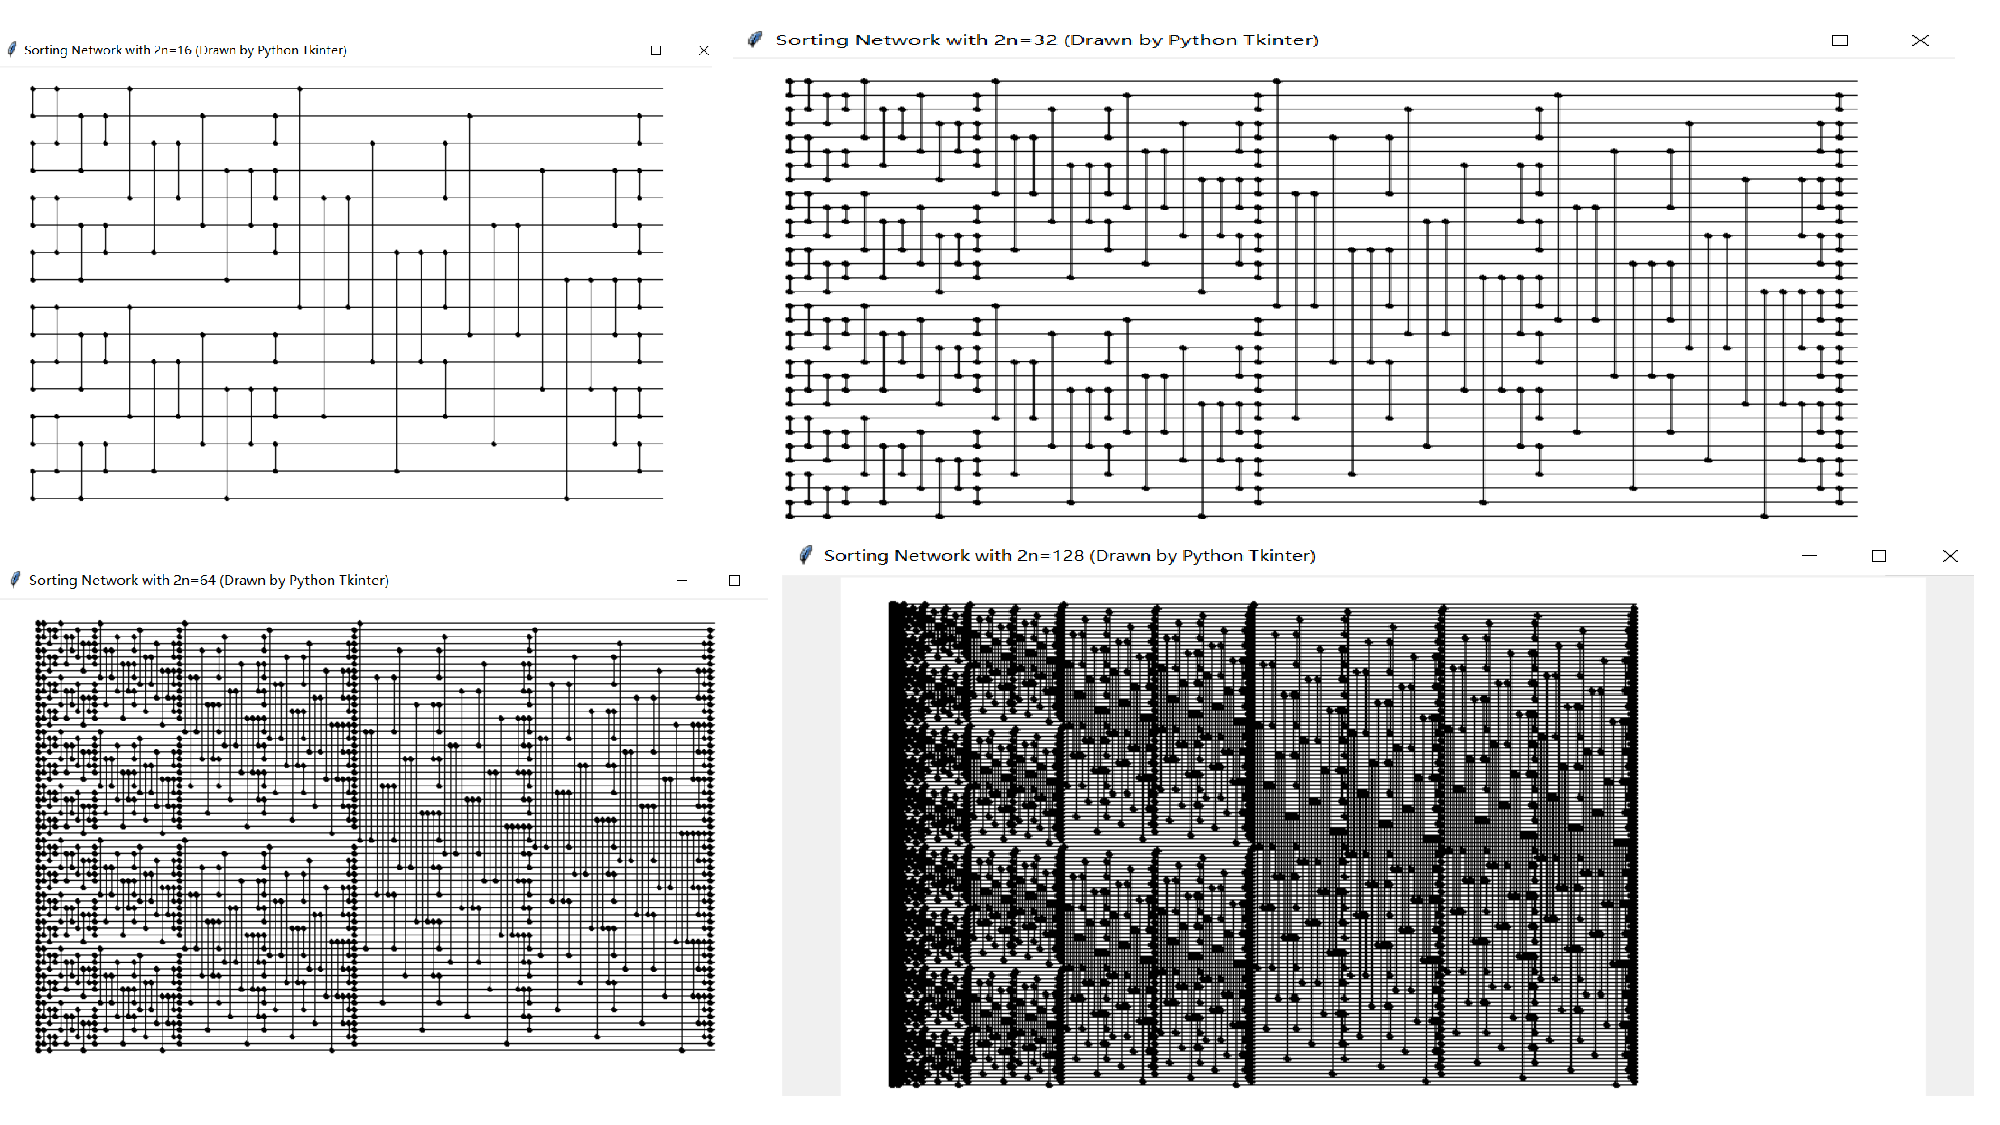
\includegraphics[scale=0.6]{batcher.pdf}
		 \caption{Fig1}
		 \label{fig1}
	\end{figure}
	\begin{proof}
	(a) The figure for $2n = 16, 32, 64, 128$ can be referred to in Fig\ref{fig1}, which are all drawn by Tkinter.
	
	(b) First we let $n = 2^k$, then we define the depth of a n-input odd-even sorting network $S(n)$ and the depth of a n-input 
	batcher's merging network $M(n)$.

	As can be seen in Fig\ref{fig2}, we can get the recurrence relation:
	
	\begin{equation*}
		S[2^k] = S[2^{k - 1}] + M[2^k]
	\end{equation*}

	\begin{equation*}
	 M[2^k] = 2M[2^{k - 1}] + 1
	\end{equation*}

	So it is easy to get: $M[2^k] = 2^k - 1$, and $S[2^k] = 2^{k + 1} - k - 2$. So for 2n-input, we can get:
	\begin{equation*}
		S[2n] = 4n - \log n - 3
	\end{equation*}
   
	\begin{figure}
		\centering
		 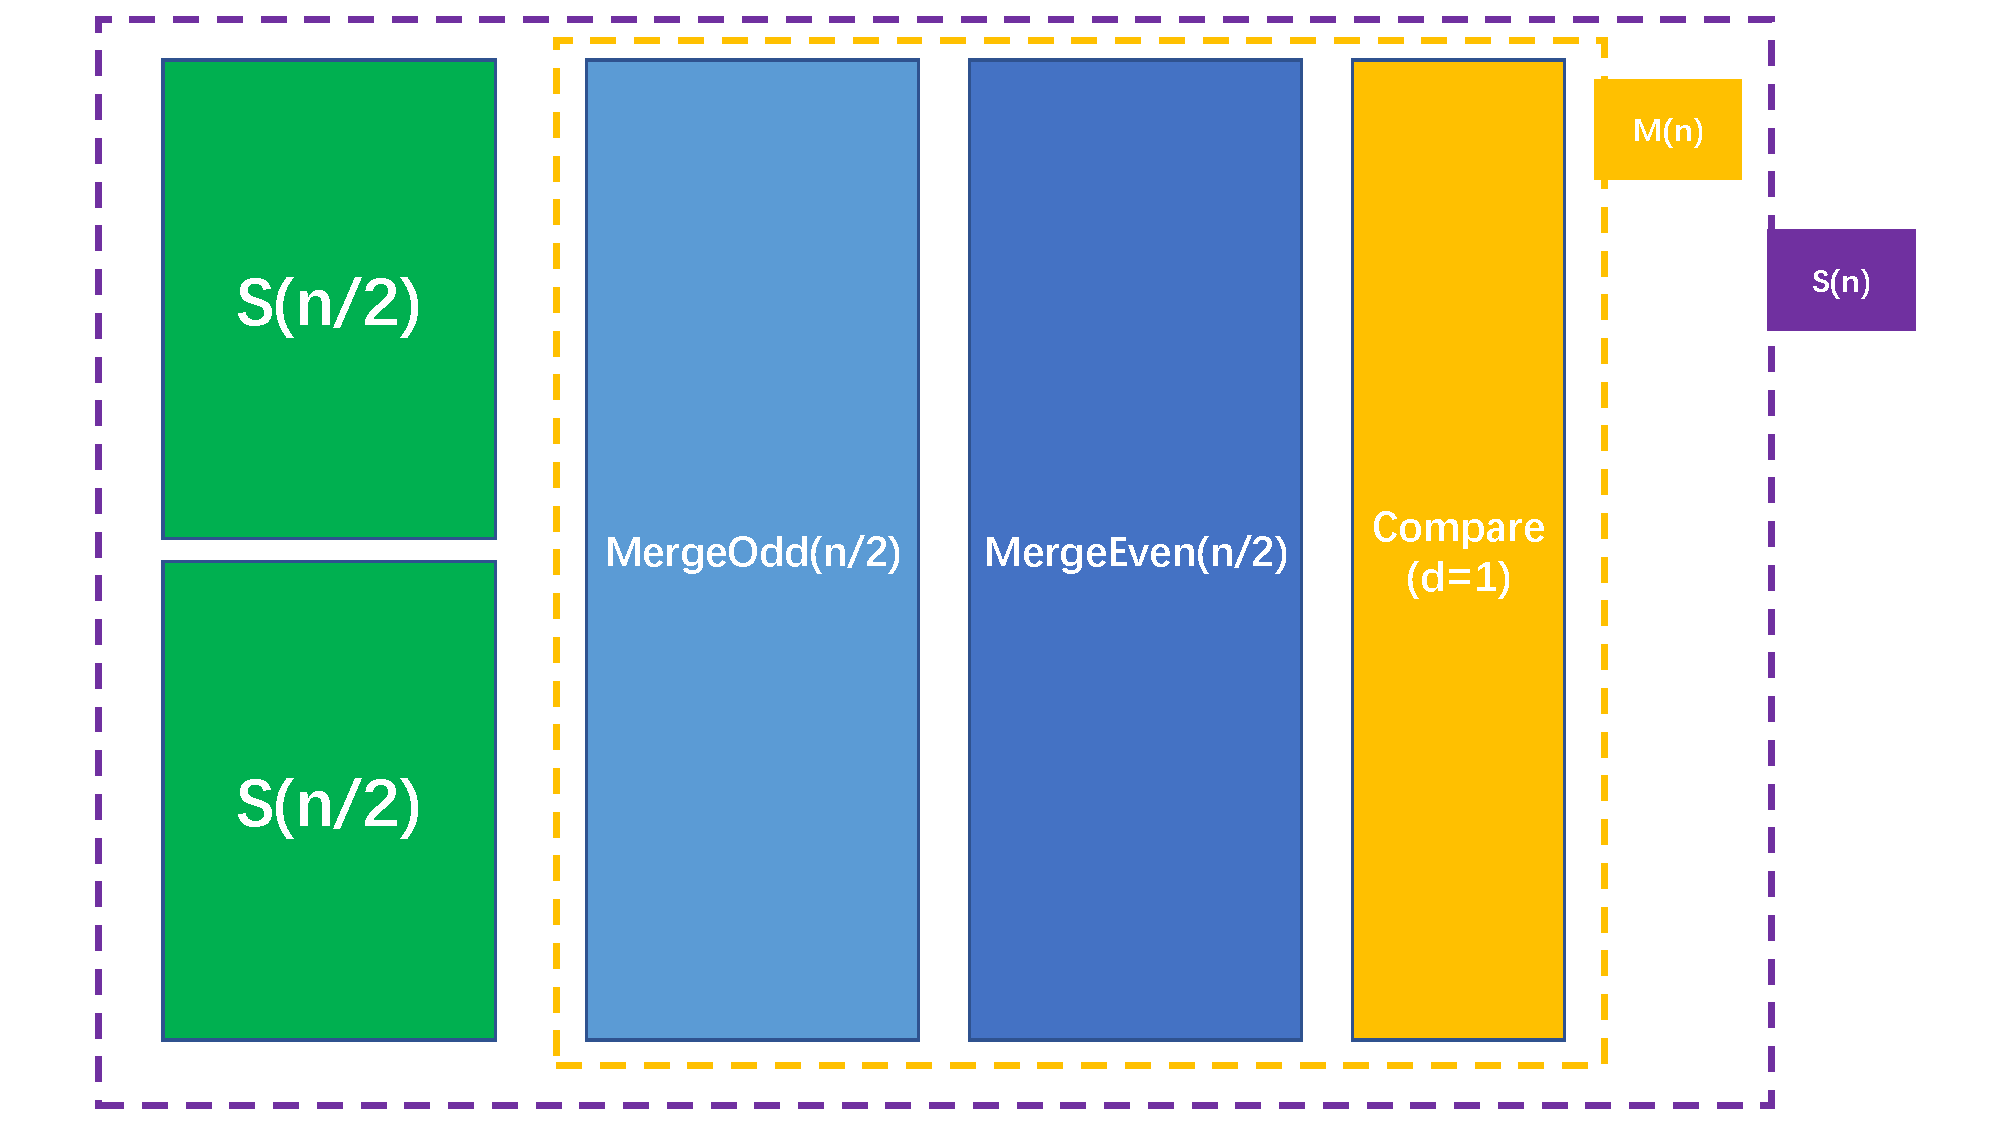
\includegraphics[scale=0.55]{Struct.pdf}
		 \caption{Fig1}
		 \label{fig2}
	\end{figure}

	(c) The merging operation can be divided into three parts: first we input two sored arrays, in the zero-one principle proof $<0, 0, ..., 0, 1, ..., 1>$, then we 
	sorted the odd and even subarray respectively, at the end we check each $a_{2i}$ and $a_{2i+1}$ as is illustrated in the context.
	 
	Actually I want to prove the correctness of the above operations by proving a more general lemma which is:
	
	\begin{lemma}
		Given two sorted arrays $<a_1, a_2, ..., a_n>$
		and $<b_1, b_2, ..., b_n>$, we respectively sort 
		$<a_1, a_3, ..., a_{n-1}, b_1, b_3, ..., b_{n-1}>$
		 and 
		$<a_2, a_4, ..., a_n, b_2, b_4, ..., b_n>$. 
		Then we can get a merged array 
		$<a_1^{'}, a_2^{'}, a_n^{'}, b_1^{'}, b_2^{'}, ..., b_n^{'}>$. 
		For simplicity we name it $<c_1, c_2, ..., c_{2n}>$, where $n=2k, k \in N$
	   , then we have:
	   
	   \begin{gather*}
		c_1 < min\{c_2, c_3\} \\
		min\{c_{2n-2}, c_{2n - 1}\} < c_{2n} \\
		max\{c_{2k}, c_{2k+1}\} < min\{c_{2k+2}, c_{2k+3}\} (k \in \{1, 2, ..., n-2\}) 
	   \end{gather*}
	\end{lemma}

	The lemma actually give an insght into why we should exchange $a_{2i}$ and $a_{2i+1}$. We can prove it by \textbf{Mathematical Induction}:

	\text{First} for $n = 2$, since $c_1 < c_3$, $c_1 = min\{a1, b1\}$ and $c_2=min\{a2, b2\}$, we can get $c_1 < min\{c_2, c_3\}$, samely: $c_4 > max\{c2, c3\}$.

	\text{Then} when $n = 2k + 2$, by induction we can get:

	\begin{gather*}
		c_1 < min\{c_2, c_3\} \\
		min\{c_{2k-2}, c_{2k - 1}\} < c_{2k} \\
		max\{c_{2j}, c_{2j+1}\} < min\{c_{2j+2}, c_{2j+3}\} (j \in \{1, 2, ..., n-2\}) 
	\end{gather*}

	
	
	we just need to prove that 



    \end{proof}

\end{enumerate}



\vspace{20pt}

\textbf{Remark:} You need to include your .pdf, .tex and .py files (or other possible sources) in your uploaded .rar or .zip file.

%========================================================================
\end{document}
